% Created by tikzDevice version 0.12.3.1 on 2022-08-25 17:19:48
% !TEX encoding = UTF-8 Unicode
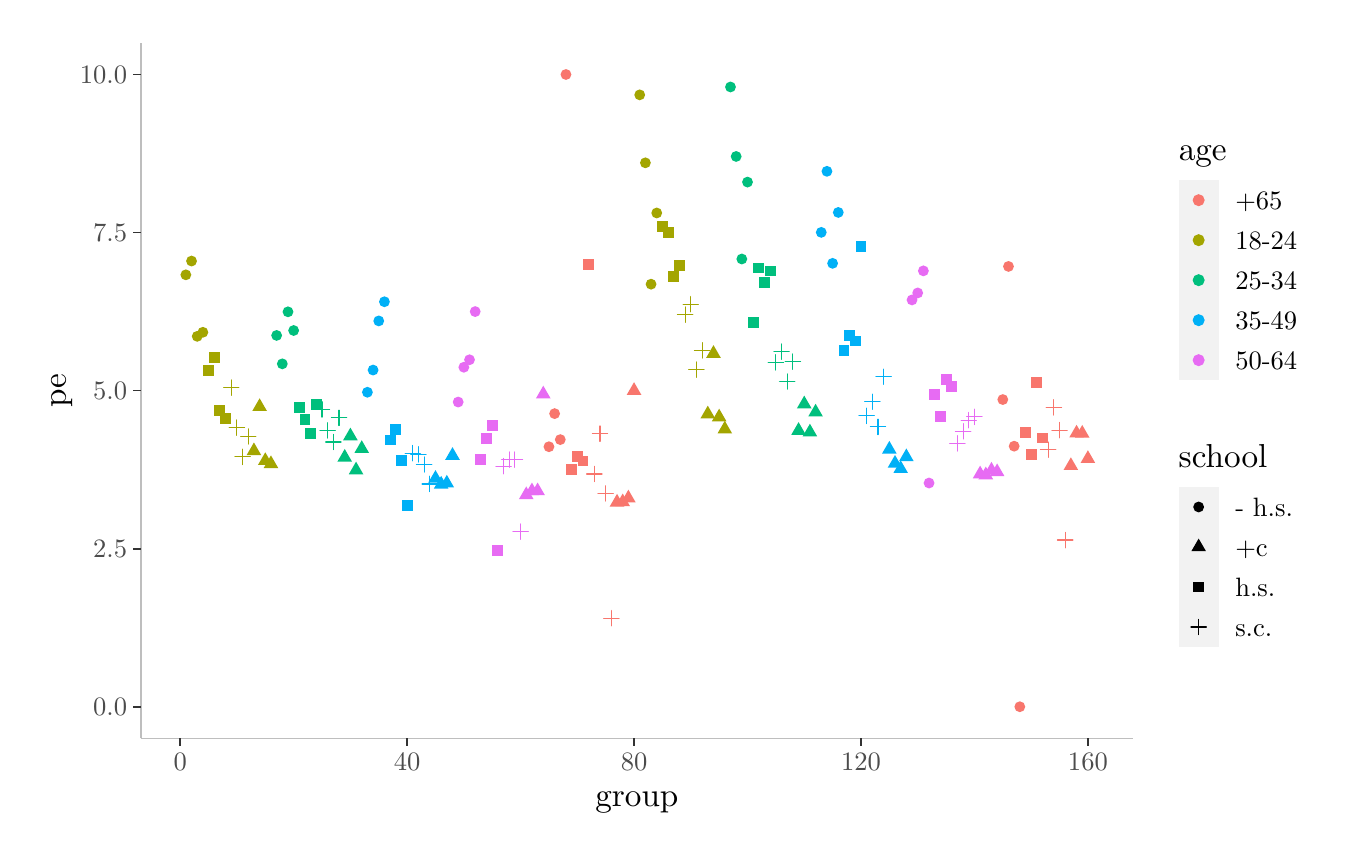
\begin{tikzpicture}[x=1pt,y=1pt]
\definecolor{fillColor}{RGB}{255,255,255}
\path[use as bounding box,fill=fillColor,fill opacity=0.00] (0,0) rectangle (469.75,289.08);
\begin{scope}
\path[clip] (  0.00,  0.00) rectangle (469.75,289.08);
\definecolor{drawColor}{RGB}{255,255,255}
\definecolor{fillColor}{RGB}{255,255,255}

\path[draw=drawColor,line width= 0.6pt,line join=round,line cap=round,fill=fillColor] (  0.00,  0.00) rectangle (469.76,289.08);
\end{scope}
\begin{scope}
\path[clip] ( 40.86, 32.28) rectangle (399.41,283.58);
\definecolor{drawColor}{RGB}{255,255,255}

\path[draw=drawColor,line width= 0.6pt,line join=round] ( 40.86, 43.70) --
	(399.41, 43.70);

\path[draw=drawColor,line width= 0.6pt,line join=round] ( 40.86,100.81) --
	(399.41,100.81);

\path[draw=drawColor,line width= 0.6pt,line join=round] ( 40.86,157.93) --
	(399.41,157.93);

\path[draw=drawColor,line width= 0.6pt,line join=round] ( 40.86,215.04) --
	(399.41,215.04);

\path[draw=drawColor,line width= 0.6pt,line join=round] ( 40.86,272.16) --
	(399.41,272.16);

\path[draw=drawColor,line width= 0.6pt,line join=round] ( 55.11, 32.28) --
	( 55.11,283.58);

\path[draw=drawColor,line width= 0.6pt,line join=round] (137.11, 32.28) --
	(137.11,283.58);

\path[draw=drawColor,line width= 0.6pt,line join=round] (219.11, 32.28) --
	(219.11,283.58);

\path[draw=drawColor,line width= 0.6pt,line join=round] (301.11, 32.28) --
	(301.11,283.58);

\path[draw=drawColor,line width= 0.6pt,line join=round] (383.11, 32.28) --
	(383.11,283.58);
\definecolor{fillColor}{RGB}{163,165,0}

\path[fill=fillColor] ( 57.16,199.77) circle (  1.96);

\path[fill=fillColor] ( 59.21,204.75) circle (  1.96);

\path[fill=fillColor] ( 61.26,177.54) circle (  1.96);

\path[fill=fillColor] ( 63.31,179.01) circle (  1.96);

\path[fill=fillColor] ( 63.40,163.34) --
	( 67.32,163.34) --
	( 67.32,167.26) --
	( 63.40,167.26) --
	cycle;

\path[fill=fillColor] ( 65.45,167.98) --
	( 69.37,167.98) --
	( 69.37,171.91) --
	( 65.45,171.91) --
	cycle;

\path[fill=fillColor] ( 67.50,148.62) --
	( 71.42,148.62) --
	( 71.42,152.55) --
	( 67.50,152.55) --
	cycle;

\path[fill=fillColor] ( 69.55,145.77) --
	( 73.47,145.77) --
	( 73.47,149.69) --
	( 69.55,149.69) --
	cycle;
\definecolor{drawColor}{RGB}{163,165,0}

\path[draw=drawColor,line width= 0.4pt,line join=round,line cap=round] ( 70.78,159.01) -- ( 76.33,159.01);

\path[draw=drawColor,line width= 0.4pt,line join=round,line cap=round] ( 73.56,156.24) -- ( 73.56,161.79);

\path[draw=drawColor,line width= 0.4pt,line join=round,line cap=round] ( 72.83,144.53) -- ( 78.38,144.53);

\path[draw=drawColor,line width= 0.4pt,line join=round,line cap=round] ( 75.61,141.76) -- ( 75.61,147.31);

\path[draw=drawColor,line width= 0.4pt,line join=round,line cap=round] ( 74.88,133.99) -- ( 80.43,133.99);

\path[draw=drawColor,line width= 0.4pt,line join=round,line cap=round] ( 77.66,131.22) -- ( 77.66,136.77);

\path[draw=drawColor,line width= 0.4pt,line join=round,line cap=round] ( 76.93,141.35) -- ( 82.48,141.35);

\path[draw=drawColor,line width= 0.4pt,line join=round,line cap=round] ( 79.71,138.58) -- ( 79.71,144.13);

\path[fill=fillColor] ( 81.76,139.19) --
	( 84.40,134.61) --
	( 79.12,134.61) --
	cycle;

\path[fill=fillColor] ( 83.81,155.16) --
	( 86.45,150.58) --
	( 81.17,150.58) --
	cycle;

\path[fill=fillColor] ( 85.86,135.65) --
	( 88.50,131.07) --
	( 83.22,131.07) --
	cycle;

\path[fill=fillColor] ( 87.91,134.52) --
	( 90.55,129.94) --
	( 85.27,129.94) --
	cycle;
\definecolor{fillColor}{RGB}{0,191,125}

\path[fill=fillColor] ( 89.96,177.87) circle (  1.96);

\path[fill=fillColor] ( 92.01,167.60) circle (  1.96);

\path[fill=fillColor] ( 94.06,186.40) circle (  1.96);

\path[fill=fillColor] ( 96.11,179.65) circle (  1.96);

\path[fill=fillColor] ( 96.20,149.73) --
	(100.12,149.73) --
	(100.12,153.65) --
	( 96.20,153.65) --
	cycle;

\path[fill=fillColor] ( 98.25,145.43) --
	(102.17,145.43) --
	(102.17,149.35) --
	( 98.25,149.35) --
	cycle;

\path[fill=fillColor] (100.30,140.50) --
	(104.22,140.50) --
	(104.22,144.42) --
	(100.30,144.42) --
	cycle;

\path[fill=fillColor] (102.35,151.06) --
	(106.27,151.06) --
	(106.27,154.98) --
	(102.35,154.98) --
	cycle;
\definecolor{drawColor}{RGB}{0,191,125}

\path[draw=drawColor,line width= 0.4pt,line join=round,line cap=round] (103.58,151.14) -- (109.13,151.14);

\path[draw=drawColor,line width= 0.4pt,line join=round,line cap=round] (106.36,148.36) -- (106.36,153.91);

\path[draw=drawColor,line width= 0.4pt,line join=round,line cap=round] (105.63,143.53) -- (111.18,143.53);

\path[draw=drawColor,line width= 0.4pt,line join=round,line cap=round] (108.41,140.76) -- (108.41,146.31);

\path[draw=drawColor,line width= 0.4pt,line join=round,line cap=round] (107.68,139.36) -- (113.23,139.36);

\path[draw=drawColor,line width= 0.4pt,line join=round,line cap=round] (110.46,136.58) -- (110.46,142.13);

\path[draw=drawColor,line width= 0.4pt,line join=round,line cap=round] (109.73,148.09) -- (115.28,148.09);

\path[draw=drawColor,line width= 0.4pt,line join=round,line cap=round] (112.51,145.31) -- (112.51,150.86);

\path[fill=fillColor] (114.56,136.85) --
	(117.20,132.27) --
	(111.92,132.27) --
	cycle;

\path[fill=fillColor] (116.61,144.57) --
	(119.25,139.99) --
	(113.97,139.99) --
	cycle;

\path[fill=fillColor] (118.66,132.26) --
	(121.30,127.68) --
	(116.02,127.68) --
	cycle;

\path[fill=fillColor] (120.71,140.00) --
	(123.35,135.42) --
	(118.07,135.42) --
	cycle;
\definecolor{fillColor}{RGB}{0,176,246}

\path[fill=fillColor] (122.76,157.34) circle (  1.96);

\path[fill=fillColor] (124.81,165.36) circle (  1.96);

\path[fill=fillColor] (126.86,183.11) circle (  1.96);

\path[fill=fillColor] (128.91,190.04) circle (  1.96);

\path[fill=fillColor] (129.00,138.11) --
	(132.92,138.11) --
	(132.92,142.03) --
	(129.00,142.03) --
	cycle;

\path[fill=fillColor] (131.05,142.03) --
	(134.97,142.03) --
	(134.97,145.96) --
	(131.05,145.96) --
	cycle;

\path[fill=fillColor] (133.10,130.56) --
	(137.02,130.56) --
	(137.02,134.49) --
	(133.10,134.49) --
	cycle;

\path[fill=fillColor] (135.15,114.38) --
	(139.07,114.38) --
	(139.07,118.31) --
	(135.15,118.31) --
	cycle;
\definecolor{drawColor}{RGB}{0,176,246}

\path[draw=drawColor,line width= 0.4pt,line join=round,line cap=round] (136.38,135.31) -- (141.93,135.31);

\path[draw=drawColor,line width= 0.4pt,line join=round,line cap=round] (139.16,132.54) -- (139.16,138.09);

\path[draw=drawColor,line width= 0.4pt,line join=round,line cap=round] (138.43,134.88) -- (143.98,134.88);

\path[draw=drawColor,line width= 0.4pt,line join=round,line cap=round] (141.21,132.10) -- (141.21,137.65);

\path[draw=drawColor,line width= 0.4pt,line join=round,line cap=round] (140.48,131.23) -- (146.03,131.23);

\path[draw=drawColor,line width= 0.4pt,line join=round,line cap=round] (143.26,128.45) -- (143.26,134.00);

\path[draw=drawColor,line width= 0.4pt,line join=round,line cap=round] (142.53,124.20) -- (148.08,124.20);

\path[draw=drawColor,line width= 0.4pt,line join=round,line cap=round] (145.31,121.43) -- (145.31,126.98);

\path[fill=fillColor] (147.36,129.22) --
	(150.00,124.64) --
	(144.72,124.64) --
	cycle;

\path[fill=fillColor] (149.41,127.11) --
	(152.05,122.53) --
	(146.77,122.53) --
	cycle;

\path[fill=fillColor] (151.46,127.49) --
	(154.10,122.92) --
	(148.82,122.92) --
	cycle;

\path[fill=fillColor] (153.51,137.52) --
	(156.15,132.94) --
	(150.87,132.94) --
	cycle;
\definecolor{fillColor}{RGB}{231,107,243}

\path[fill=fillColor] (155.56,153.80) circle (  1.96);

\path[fill=fillColor] (157.61,166.37) circle (  1.96);

\path[fill=fillColor] (159.66,169.08) circle (  1.96);

\path[fill=fillColor] (161.71,186.49) circle (  1.96);

\path[fill=fillColor] (161.80,130.96) --
	(165.72,130.96) --
	(165.72,134.88) --
	(161.80,134.88) --
	cycle;

\path[fill=fillColor] (163.85,138.52) --
	(167.77,138.52) --
	(167.77,142.44) --
	(163.85,142.44) --
	cycle;

\path[fill=fillColor] (165.90,143.36) --
	(169.82,143.36) --
	(169.82,147.29) --
	(165.90,147.29) --
	cycle;

\path[fill=fillColor] (167.95, 98.18) --
	(171.87, 98.18) --
	(171.87,102.10) --
	(167.95,102.10) --
	cycle;
\definecolor{drawColor}{RGB}{231,107,243}

\path[draw=drawColor,line width= 0.4pt,line join=round,line cap=round] (169.18,130.63) -- (174.73,130.63);

\path[draw=drawColor,line width= 0.4pt,line join=round,line cap=round] (171.96,127.86) -- (171.96,133.41);

\path[draw=drawColor,line width= 0.4pt,line join=round,line cap=round] (171.23,133.00) -- (176.78,133.00);

\path[draw=drawColor,line width= 0.4pt,line join=round,line cap=round] (174.01,130.23) -- (174.01,135.78);

\path[draw=drawColor,line width= 0.4pt,line join=round,line cap=round] (173.28,132.99) -- (178.83,132.99);

\path[draw=drawColor,line width= 0.4pt,line join=round,line cap=round] (176.06,130.22) -- (176.06,135.77);

\path[draw=drawColor,line width= 0.4pt,line join=round,line cap=round] (175.33,106.96) -- (180.88,106.96);

\path[draw=drawColor,line width= 0.4pt,line join=round,line cap=round] (178.11,104.19) -- (178.11,109.74);

\path[fill=fillColor] (180.16,123.30) --
	(182.80,118.72) --
	(177.52,118.72) --
	cycle;

\path[fill=fillColor] (182.21,124.70) --
	(184.85,120.12) --
	(179.57,120.12) --
	cycle;

\path[fill=fillColor] (184.26,124.72) --
	(186.90,120.14) --
	(181.62,120.14) --
	cycle;

\path[fill=fillColor] (186.31,159.71) --
	(188.95,155.13) --
	(183.67,155.13) --
	cycle;
\definecolor{fillColor}{RGB}{248,118,109}

\path[fill=fillColor] (188.36,137.65) circle (  1.96);

\path[fill=fillColor] (190.41,149.62) circle (  1.96);

\path[fill=fillColor] (192.46,140.23) circle (  1.96);

\path[fill=fillColor] (194.51,272.16) circle (  1.96);

\path[fill=fillColor] (194.60,127.32) --
	(198.52,127.32) --
	(198.52,131.25) --
	(194.60,131.25) --
	cycle;

\path[fill=fillColor] (196.65,132.03) --
	(200.57,132.03) --
	(200.57,135.95) --
	(196.65,135.95) --
	cycle;

\path[fill=fillColor] (198.70,130.51) --
	(202.62,130.51) --
	(202.62,134.44) --
	(198.70,134.44) --
	cycle;

\path[fill=fillColor] (200.75,201.66) --
	(204.67,201.66) --
	(204.67,205.58) --
	(200.75,205.58) --
	cycle;
\definecolor{drawColor}{RGB}{248,118,109}

\path[draw=drawColor,line width= 0.4pt,line join=round,line cap=round] (201.98,127.81) -- (207.53,127.81);

\path[draw=drawColor,line width= 0.4pt,line join=round,line cap=round] (204.76,125.03) -- (204.76,130.58);

\path[draw=drawColor,line width= 0.4pt,line join=round,line cap=round] (204.03,142.36) -- (209.58,142.36);

\path[draw=drawColor,line width= 0.4pt,line join=round,line cap=round] (206.81,139.59) -- (206.81,145.14);

\path[draw=drawColor,line width= 0.4pt,line join=round,line cap=round] (206.08,120.77) -- (211.63,120.77);

\path[draw=drawColor,line width= 0.4pt,line join=round,line cap=round] (208.86,117.99) -- (208.86,123.54);

\path[draw=drawColor,line width= 0.4pt,line join=round,line cap=round] (208.13, 75.68) -- (213.68, 75.68);

\path[draw=drawColor,line width= 0.4pt,line join=round,line cap=round] (210.91, 72.91) -- (210.91, 78.46);

\path[fill=fillColor] (212.96,120.63) --
	(215.60,116.05) --
	(210.32,116.05) --
	cycle;

\path[fill=fillColor] (215.01,120.75) --
	(217.65,116.17) --
	(212.37,116.17) --
	cycle;

\path[fill=fillColor] (217.06,122.12) --
	(219.70,117.54) --
	(214.42,117.54) --
	cycle;

\path[fill=fillColor] (219.11,160.98) --
	(221.75,156.40) --
	(216.47,156.40) --
	cycle;
\definecolor{fillColor}{RGB}{163,165,0}

\path[fill=fillColor] (221.16,264.80) circle (  1.96);

\path[fill=fillColor] (223.21,240.24) circle (  1.96);

\path[fill=fillColor] (225.26,196.39) circle (  1.96);

\path[fill=fillColor] (227.31,222.12) circle (  1.96);

\path[fill=fillColor] (227.40,215.35) --
	(231.32,215.35) --
	(231.32,219.27) --
	(227.40,219.27) --
	cycle;

\path[fill=fillColor] (229.45,213.14) --
	(233.37,213.14) --
	(233.37,217.07) --
	(229.45,217.07) --
	cycle;

\path[fill=fillColor] (231.50,197.10) --
	(235.42,197.10) --
	(235.42,201.03) --
	(231.50,201.03) --
	cycle;

\path[fill=fillColor] (233.55,201.12) --
	(237.47,201.12) --
	(237.47,205.05) --
	(233.55,205.05) --
	cycle;
\definecolor{drawColor}{RGB}{163,165,0}

\path[draw=drawColor,line width= 0.4pt,line join=round,line cap=round] (234.78,185.41) -- (240.33,185.41);

\path[draw=drawColor,line width= 0.4pt,line join=round,line cap=round] (237.56,182.63) -- (237.56,188.18);

\path[draw=drawColor,line width= 0.4pt,line join=round,line cap=round] (236.83,189.15) -- (242.38,189.15);

\path[draw=drawColor,line width= 0.4pt,line join=round,line cap=round] (239.61,186.37) -- (239.61,191.92);

\path[draw=drawColor,line width= 0.4pt,line join=round,line cap=round] (238.88,165.52) -- (244.43,165.52);

\path[draw=drawColor,line width= 0.4pt,line join=round,line cap=round] (241.66,162.75) -- (241.66,168.30);

\path[draw=drawColor,line width= 0.4pt,line join=round,line cap=round] (240.93,172.50) -- (246.48,172.50);

\path[draw=drawColor,line width= 0.4pt,line join=round,line cap=round] (243.71,169.72) -- (243.71,175.27);

\path[fill=fillColor] (245.76,152.49) --
	(248.40,147.92) --
	(243.12,147.92) --
	cycle;

\path[fill=fillColor] (247.81,174.37) --
	(250.45,169.79) --
	(245.17,169.79) --
	cycle;

\path[fill=fillColor] (249.86,151.41) --
	(252.50,146.83) --
	(247.22,146.83) --
	cycle;

\path[fill=fillColor] (251.91,147.04) --
	(254.55,142.46) --
	(249.27,142.46) --
	cycle;
\definecolor{fillColor}{RGB}{0,191,125}

\path[fill=fillColor] (253.96,267.65) circle (  1.96);

\path[fill=fillColor] (256.01,242.54) circle (  1.96);

\path[fill=fillColor] (258.06,205.49) circle (  1.96);

\path[fill=fillColor] (260.11,233.28) circle (  1.96);

\path[fill=fillColor] (260.20,180.57) --
	(264.12,180.57) --
	(264.12,184.49) --
	(260.20,184.49) --
	cycle;

\path[fill=fillColor] (262.25,200.29) --
	(266.17,200.29) --
	(266.17,204.21) --
	(262.25,204.21) --
	cycle;

\path[fill=fillColor] (264.30,194.90) --
	(268.22,194.90) --
	(268.22,198.82) --
	(264.30,198.82) --
	cycle;

\path[fill=fillColor] (266.35,199.20) --
	(270.27,199.20) --
	(270.27,203.13) --
	(266.35,203.13) --
	cycle;
\definecolor{drawColor}{RGB}{0,191,125}

\path[draw=drawColor,line width= 0.4pt,line join=round,line cap=round] (267.58,168.13) -- (273.13,168.13);

\path[draw=drawColor,line width= 0.4pt,line join=round,line cap=round] (270.36,165.36) -- (270.36,170.91);

\path[draw=drawColor,line width= 0.4pt,line join=round,line cap=round] (269.63,172.01) -- (275.18,172.01);

\path[draw=drawColor,line width= 0.4pt,line join=round,line cap=round] (272.41,169.24) -- (272.41,174.79);

\path[draw=drawColor,line width= 0.4pt,line join=round,line cap=round] (271.68,161.21) -- (277.23,161.21);

\path[draw=drawColor,line width= 0.4pt,line join=round,line cap=round] (274.46,158.44) -- (274.46,163.99);

\path[draw=drawColor,line width= 0.4pt,line join=round,line cap=round] (273.73,168.42) -- (279.28,168.42);

\path[draw=drawColor,line width= 0.4pt,line join=round,line cap=round] (276.51,165.64) -- (276.51,171.19);

\path[fill=fillColor] (278.56,146.54) --
	(281.20,141.96) --
	(275.92,141.96) --
	cycle;

\path[fill=fillColor] (280.61,156.12) --
	(283.25,151.54) --
	(277.97,151.54) --
	cycle;

\path[fill=fillColor] (282.66,145.96) --
	(285.30,141.38) --
	(280.02,141.38) --
	cycle;

\path[fill=fillColor] (284.71,153.17) --
	(287.35,148.59) --
	(282.07,148.59) --
	cycle;
\definecolor{fillColor}{RGB}{0,176,246}

\path[fill=fillColor] (286.76,215.11) circle (  1.96);

\path[fill=fillColor] (288.81,237.17) circle (  1.96);

\path[fill=fillColor] (290.86,203.92) circle (  1.96);

\path[fill=fillColor] (292.91,222.31) circle (  1.96);

\path[fill=fillColor] (293.00,170.60) --
	(296.92,170.60) --
	(296.92,174.52) --
	(293.00,174.52) --
	cycle;

\path[fill=fillColor] (295.05,175.91) --
	(298.97,175.91) --
	(298.97,179.84) --
	(295.05,179.84) --
	cycle;

\path[fill=fillColor] (297.10,173.90) --
	(301.02,173.90) --
	(301.02,177.83) --
	(297.10,177.83) --
	cycle;

\path[fill=fillColor] (299.15,207.90) --
	(303.07,207.90) --
	(303.07,211.82) --
	(299.15,211.82) --
	cycle;
\definecolor{drawColor}{RGB}{0,176,246}

\path[draw=drawColor,line width= 0.4pt,line join=round,line cap=round] (300.38,148.81) -- (305.93,148.81);

\path[draw=drawColor,line width= 0.4pt,line join=round,line cap=round] (303.16,146.03) -- (303.16,151.58);

\path[draw=drawColor,line width= 0.4pt,line join=round,line cap=round] (302.43,153.91) -- (307.98,153.91);

\path[draw=drawColor,line width= 0.4pt,line join=round,line cap=round] (305.21,151.13) -- (305.21,156.68);

\path[draw=drawColor,line width= 0.4pt,line join=round,line cap=round] (304.48,144.81) -- (310.03,144.81);

\path[draw=drawColor,line width= 0.4pt,line join=round,line cap=round] (307.26,142.03) -- (307.26,147.58);

\path[draw=drawColor,line width= 0.4pt,line join=round,line cap=round] (306.53,162.93) -- (312.08,162.93);

\path[draw=drawColor,line width= 0.4pt,line join=round,line cap=round] (309.31,160.16) -- (309.31,165.70);

\path[fill=fillColor] (311.36,139.75) --
	(314.00,135.18) --
	(308.72,135.18) --
	cycle;

\path[fill=fillColor] (313.41,134.67) --
	(316.05,130.10) --
	(310.77,130.10) --
	cycle;

\path[fill=fillColor] (315.46,132.73) --
	(318.10,128.16) --
	(312.82,128.16) --
	cycle;

\path[fill=fillColor] (317.51,137.02) --
	(320.15,132.44) --
	(314.87,132.44) --
	cycle;
\definecolor{fillColor}{RGB}{231,107,243}

\path[fill=fillColor] (319.56,190.70) circle (  1.96);

\path[fill=fillColor] (321.61,193.22) circle (  1.96);

\path[fill=fillColor] (323.66,201.20) circle (  1.96);

\path[fill=fillColor] (325.71,124.54) circle (  1.96);

\path[fill=fillColor] (325.80,154.52) --
	(329.72,154.52) --
	(329.72,158.45) --
	(325.80,158.45) --
	cycle;

\path[fill=fillColor] (327.85,146.71) --
	(331.77,146.71) --
	(331.77,150.63) --
	(327.85,150.63) --
	cycle;

\path[fill=fillColor] (329.90,160.00) --
	(333.82,160.00) --
	(333.82,163.93) --
	(329.90,163.93) --
	cycle;

\path[fill=fillColor] (331.95,157.39) --
	(335.87,157.39) --
	(335.87,161.32) --
	(331.95,161.32) --
	cycle;
\definecolor{drawColor}{RGB}{231,107,243}

\path[draw=drawColor,line width= 0.4pt,line join=round,line cap=round] (333.18,138.87) -- (338.73,138.87);

\path[draw=drawColor,line width= 0.4pt,line join=round,line cap=round] (335.96,136.10) -- (335.96,141.65);

\path[draw=drawColor,line width= 0.4pt,line join=round,line cap=round] (335.23,143.23) -- (340.78,143.23);

\path[draw=drawColor,line width= 0.4pt,line join=round,line cap=round] (338.01,140.46) -- (338.01,146.01);

\path[draw=drawColor,line width= 0.4pt,line join=round,line cap=round] (337.28,147.24) -- (342.83,147.24);

\path[draw=drawColor,line width= 0.4pt,line join=round,line cap=round] (340.06,144.46) -- (340.06,150.01);

\path[draw=drawColor,line width= 0.4pt,line join=round,line cap=round] (339.33,148.45) -- (344.88,148.45);

\path[draw=drawColor,line width= 0.4pt,line join=round,line cap=round] (342.11,145.68) -- (342.11,151.23);

\path[fill=fillColor] (344.16,130.82) --
	(346.80,126.24) --
	(341.52,126.24) --
	cycle;

\path[fill=fillColor] (346.21,130.48) --
	(348.85,125.90) --
	(343.57,125.90) --
	cycle;

\path[fill=fillColor] (348.26,132.18) --
	(350.90,127.61) --
	(345.62,127.61) --
	cycle;

\path[fill=fillColor] (350.31,131.61) --
	(352.95,127.03) --
	(347.67,127.03) --
	cycle;
\definecolor{fillColor}{RGB}{248,118,109}

\path[fill=fillColor] (352.36,154.70) circle (  1.96);

\path[fill=fillColor] (354.41,202.80) circle (  1.96);

\path[fill=fillColor] (356.46,137.85) circle (  1.96);

\path[fill=fillColor] (358.51, 43.70) circle (  1.96);

\path[fill=fillColor] (358.60,140.85) --
	(362.52,140.85) --
	(362.52,144.77) --
	(358.60,144.77) --
	cycle;

\path[fill=fillColor] (360.65,132.94) --
	(364.57,132.94) --
	(364.57,136.87) --
	(360.65,136.87) --
	cycle;

\path[fill=fillColor] (362.70,158.82) --
	(366.62,158.82) --
	(366.62,162.75) --
	(362.70,162.75) --
	cycle;

\path[fill=fillColor] (364.75,138.83) --
	(368.67,138.83) --
	(368.67,142.76) --
	(364.75,142.76) --
	cycle;
\definecolor{drawColor}{RGB}{248,118,109}

\path[draw=drawColor,line width= 0.4pt,line join=round,line cap=round] (365.98,136.58) -- (371.53,136.58);

\path[draw=drawColor,line width= 0.4pt,line join=round,line cap=round] (368.76,133.80) -- (368.76,139.35);

\path[draw=drawColor,line width= 0.4pt,line join=round,line cap=round] (368.03,151.86) -- (373.58,151.86);

\path[draw=drawColor,line width= 0.4pt,line join=round,line cap=round] (370.81,149.08) -- (370.81,154.63);

\path[draw=drawColor,line width= 0.4pt,line join=round,line cap=round] (370.08,143.66) -- (375.63,143.66);

\path[draw=drawColor,line width= 0.4pt,line join=round,line cap=round] (372.86,140.89) -- (372.86,146.44);

\path[draw=drawColor,line width= 0.4pt,line join=round,line cap=round] (372.13,103.93) -- (377.68,103.93);

\path[draw=drawColor,line width= 0.4pt,line join=round,line cap=round] (374.91,101.15) -- (374.91,106.70);

\path[fill=fillColor] (376.96,133.83) --
	(379.60,129.26) --
	(374.32,129.26) --
	cycle;

\path[fill=fillColor] (379.01,145.57) --
	(381.65,141.00) --
	(376.37,141.00) --
	cycle;

\path[fill=fillColor] (381.06,145.51) --
	(383.70,140.93) --
	(378.42,140.93) --
	cycle;

\path[fill=fillColor] (383.11,136.38) --
	(385.75,131.80) --
	(380.47,131.80) --
	cycle;
\end{scope}
\begin{scope}
\path[clip] (  0.00,  0.00) rectangle (469.75,289.08);
\definecolor{drawColor}{RGB}{190,190,190}

\path[draw=drawColor,line width= 0.6pt,line join=round] ( 40.86, 32.28) --
	( 40.86,283.58);
\end{scope}
\begin{scope}
\path[clip] (  0.00,  0.00) rectangle (469.75,289.08);
\definecolor{drawColor}{gray}{0.30}

\node[text=drawColor,anchor=base east,inner sep=0pt, outer sep=0pt, scale=  0.96] at ( 35.91, 40.39) {0.0};

\node[text=drawColor,anchor=base east,inner sep=0pt, outer sep=0pt, scale=  0.96] at ( 35.91, 97.51) {2.5};

\node[text=drawColor,anchor=base east,inner sep=0pt, outer sep=0pt, scale=  0.96] at ( 35.91,154.62) {5.0};

\node[text=drawColor,anchor=base east,inner sep=0pt, outer sep=0pt, scale=  0.96] at ( 35.91,211.74) {7.5};

\node[text=drawColor,anchor=base east,inner sep=0pt, outer sep=0pt, scale=  0.96] at ( 35.91,268.85) {10.0};
\end{scope}
\begin{scope}
\path[clip] (  0.00,  0.00) rectangle (469.75,289.08);
\definecolor{drawColor}{gray}{0.20}

\path[draw=drawColor,line width= 0.6pt,line join=round] ( 38.11, 43.70) --
	( 40.86, 43.70);

\path[draw=drawColor,line width= 0.6pt,line join=round] ( 38.11,100.81) --
	( 40.86,100.81);

\path[draw=drawColor,line width= 0.6pt,line join=round] ( 38.11,157.93) --
	( 40.86,157.93);

\path[draw=drawColor,line width= 0.6pt,line join=round] ( 38.11,215.04) --
	( 40.86,215.04);

\path[draw=drawColor,line width= 0.6pt,line join=round] ( 38.11,272.16) --
	( 40.86,272.16);
\end{scope}
\begin{scope}
\path[clip] (  0.00,  0.00) rectangle (469.75,289.08);
\definecolor{drawColor}{RGB}{190,190,190}

\path[draw=drawColor,line width= 0.6pt,line join=round] ( 40.86, 32.28) --
	(399.41, 32.28);
\end{scope}
\begin{scope}
\path[clip] (  0.00,  0.00) rectangle (469.75,289.08);
\definecolor{drawColor}{gray}{0.20}

\path[draw=drawColor,line width= 0.6pt,line join=round] ( 55.11, 29.53) --
	( 55.11, 32.28);

\path[draw=drawColor,line width= 0.6pt,line join=round] (137.11, 29.53) --
	(137.11, 32.28);

\path[draw=drawColor,line width= 0.6pt,line join=round] (219.11, 29.53) --
	(219.11, 32.28);

\path[draw=drawColor,line width= 0.6pt,line join=round] (301.11, 29.53) --
	(301.11, 32.28);

\path[draw=drawColor,line width= 0.6pt,line join=round] (383.11, 29.53) --
	(383.11, 32.28);
\end{scope}
\begin{scope}
\path[clip] (  0.00,  0.00) rectangle (469.75,289.08);
\definecolor{drawColor}{gray}{0.30}

\node[text=drawColor,anchor=base,inner sep=0pt, outer sep=0pt, scale=  0.96] at ( 55.11, 20.71) {0};

\node[text=drawColor,anchor=base,inner sep=0pt, outer sep=0pt, scale=  0.96] at (137.11, 20.71) {40};

\node[text=drawColor,anchor=base,inner sep=0pt, outer sep=0pt, scale=  0.96] at (219.11, 20.71) {80};

\node[text=drawColor,anchor=base,inner sep=0pt, outer sep=0pt, scale=  0.96] at (301.11, 20.71) {120};

\node[text=drawColor,anchor=base,inner sep=0pt, outer sep=0pt, scale=  0.96] at (383.11, 20.71) {160};
\end{scope}
\begin{scope}
\path[clip] (  0.00,  0.00) rectangle (469.75,289.08);
\definecolor{drawColor}{RGB}{0,0,0}

\node[text=drawColor,anchor=base,inner sep=0pt, outer sep=0pt, scale=  1.20] at (220.13,  7.83) {group};
\end{scope}
\begin{scope}
\path[clip] (  0.00,  0.00) rectangle (469.75,289.08);
\definecolor{drawColor}{RGB}{0,0,0}

\node[text=drawColor,rotate= 90.00,anchor=base,inner sep=0pt, outer sep=0pt, scale=  1.20] at ( 13.76,157.93) {pe };
\end{scope}
\begin{scope}
\path[clip] (  0.00,  0.00) rectangle (469.75,289.08);
\definecolor{fillColor}{RGB}{255,255,255}

\path[fill=fillColor] (410.41,156.20) rectangle (464.25,256.07);
\end{scope}
\begin{scope}
\path[clip] (  0.00,  0.00) rectangle (469.75,289.08);
\definecolor{drawColor}{RGB}{0,0,0}

\node[text=drawColor,anchor=base west,inner sep=0pt, outer sep=0pt, scale=  1.20] at (415.91,241.14) {age};
\end{scope}
\begin{scope}
\path[clip] (  0.00,  0.00) rectangle (469.75,289.08);
\definecolor{fillColor}{gray}{0.95}

\path[fill=fillColor] (415.91,219.52) rectangle (430.36,233.97);
\end{scope}
\begin{scope}
\path[clip] (  0.00,  0.00) rectangle (469.75,289.08);
\definecolor{drawColor}{RGB}{248,118,109}
\definecolor{fillColor}{RGB}{248,118,109}

\path[draw=drawColor,line width= 0.4pt,line join=round,line cap=round,fill=fillColor] (423.13,226.74) circle (  1.96);
\end{scope}
\begin{scope}
\path[clip] (  0.00,  0.00) rectangle (469.75,289.08);
\definecolor{fillColor}{gray}{0.95}

\path[fill=fillColor] (415.91,205.06) rectangle (430.36,219.52);
\end{scope}
\begin{scope}
\path[clip] (  0.00,  0.00) rectangle (469.75,289.08);
\definecolor{drawColor}{RGB}{163,165,0}
\definecolor{fillColor}{RGB}{163,165,0}

\path[draw=drawColor,line width= 0.4pt,line join=round,line cap=round,fill=fillColor] (423.13,212.29) circle (  1.96);
\end{scope}
\begin{scope}
\path[clip] (  0.00,  0.00) rectangle (469.75,289.08);
\definecolor{fillColor}{gray}{0.95}

\path[fill=fillColor] (415.91,190.61) rectangle (430.36,205.06);
\end{scope}
\begin{scope}
\path[clip] (  0.00,  0.00) rectangle (469.75,289.08);
\definecolor{drawColor}{RGB}{0,191,125}
\definecolor{fillColor}{RGB}{0,191,125}

\path[draw=drawColor,line width= 0.4pt,line join=round,line cap=round,fill=fillColor] (423.13,197.84) circle (  1.96);
\end{scope}
\begin{scope}
\path[clip] (  0.00,  0.00) rectangle (469.75,289.08);
\definecolor{fillColor}{gray}{0.95}

\path[fill=fillColor] (415.91,176.15) rectangle (430.36,190.61);
\end{scope}
\begin{scope}
\path[clip] (  0.00,  0.00) rectangle (469.75,289.08);
\definecolor{drawColor}{RGB}{0,176,246}
\definecolor{fillColor}{RGB}{0,176,246}

\path[draw=drawColor,line width= 0.4pt,line join=round,line cap=round,fill=fillColor] (423.13,183.38) circle (  1.96);
\end{scope}
\begin{scope}
\path[clip] (  0.00,  0.00) rectangle (469.75,289.08);
\definecolor{fillColor}{gray}{0.95}

\path[fill=fillColor] (415.91,161.70) rectangle (430.36,176.15);
\end{scope}
\begin{scope}
\path[clip] (  0.00,  0.00) rectangle (469.75,289.08);
\definecolor{drawColor}{RGB}{231,107,243}
\definecolor{fillColor}{RGB}{231,107,243}

\path[draw=drawColor,line width= 0.4pt,line join=round,line cap=round,fill=fillColor] (423.13,168.93) circle (  1.96);
\end{scope}
\begin{scope}
\path[clip] (  0.00,  0.00) rectangle (469.75,289.08);
\definecolor{drawColor}{RGB}{0,0,0}

\node[text=drawColor,anchor=base west,inner sep=0pt, outer sep=0pt, scale=  0.96] at (436.36,223.44) {+65};
\end{scope}
\begin{scope}
\path[clip] (  0.00,  0.00) rectangle (469.75,289.08);
\definecolor{drawColor}{RGB}{0,0,0}

\node[text=drawColor,anchor=base west,inner sep=0pt, outer sep=0pt, scale=  0.96] at (436.36,208.98) {18-24};
\end{scope}
\begin{scope}
\path[clip] (  0.00,  0.00) rectangle (469.75,289.08);
\definecolor{drawColor}{RGB}{0,0,0}

\node[text=drawColor,anchor=base west,inner sep=0pt, outer sep=0pt, scale=  0.96] at (436.36,194.53) {25-34};
\end{scope}
\begin{scope}
\path[clip] (  0.00,  0.00) rectangle (469.75,289.08);
\definecolor{drawColor}{RGB}{0,0,0}

\node[text=drawColor,anchor=base west,inner sep=0pt, outer sep=0pt, scale=  0.96] at (436.36,180.08) {35-49};
\end{scope}
\begin{scope}
\path[clip] (  0.00,  0.00) rectangle (469.75,289.08);
\definecolor{drawColor}{RGB}{0,0,0}

\node[text=drawColor,anchor=base west,inner sep=0pt, outer sep=0pt, scale=  0.96] at (436.36,165.62) {50-64};
\end{scope}
\begin{scope}
\path[clip] (  0.00,  0.00) rectangle (469.75,289.08);
\definecolor{fillColor}{RGB}{255,255,255}

\path[fill=fillColor] (410.41, 59.79) rectangle (462.71,145.20);
\end{scope}
\begin{scope}
\path[clip] (  0.00,  0.00) rectangle (469.75,289.08);
\definecolor{drawColor}{RGB}{0,0,0}

\node[text=drawColor,anchor=base west,inner sep=0pt, outer sep=0pt, scale=  1.20] at (415.91,130.27) {school};
\end{scope}
\begin{scope}
\path[clip] (  0.00,  0.00) rectangle (469.75,289.08);
\definecolor{fillColor}{gray}{0.95}

\path[fill=fillColor] (415.91,108.65) rectangle (430.36,123.10);
\end{scope}
\begin{scope}
\path[clip] (  0.00,  0.00) rectangle (469.75,289.08);
\definecolor{fillColor}{RGB}{0,0,0}

\path[fill=fillColor] (423.13,115.88) circle (  1.96);
\end{scope}
\begin{scope}
\path[clip] (  0.00,  0.00) rectangle (469.75,289.08);
\definecolor{fillColor}{gray}{0.95}

\path[fill=fillColor] (415.91, 94.20) rectangle (430.36,108.65);
\end{scope}
\begin{scope}
\path[clip] (  0.00,  0.00) rectangle (469.75,289.08);
\definecolor{fillColor}{RGB}{0,0,0}

\path[fill=fillColor] (423.13,104.47) --
	(425.78, 99.90) --
	(420.49, 99.90) --
	cycle;
\end{scope}
\begin{scope}
\path[clip] (  0.00,  0.00) rectangle (469.75,289.08);
\definecolor{fillColor}{gray}{0.95}

\path[fill=fillColor] (415.91, 79.74) rectangle (430.36, 94.20);
\end{scope}
\begin{scope}
\path[clip] (  0.00,  0.00) rectangle (469.75,289.08);
\definecolor{fillColor}{RGB}{0,0,0}

\path[fill=fillColor] (421.17, 85.01) --
	(425.10, 85.01) --
	(425.10, 88.93) --
	(421.17, 88.93) --
	cycle;
\end{scope}
\begin{scope}
\path[clip] (  0.00,  0.00) rectangle (469.75,289.08);
\definecolor{fillColor}{gray}{0.95}

\path[fill=fillColor] (415.91, 65.29) rectangle (430.36, 79.74);
\end{scope}
\begin{scope}
\path[clip] (  0.00,  0.00) rectangle (469.75,289.08);
\definecolor{drawColor}{RGB}{0,0,0}

\path[draw=drawColor,line width= 0.4pt,line join=round,line cap=round] (420.36, 72.51) -- (425.91, 72.51);

\path[draw=drawColor,line width= 0.4pt,line join=round,line cap=round] (423.13, 69.74) -- (423.13, 75.29);
\end{scope}
\begin{scope}
\path[clip] (  0.00,  0.00) rectangle (469.75,289.08);
\definecolor{drawColor}{RGB}{0,0,0}

\node[text=drawColor,anchor=base west,inner sep=0pt, outer sep=0pt, scale=  0.96] at (436.36,112.57) {- h.s.};
\end{scope}
\begin{scope}
\path[clip] (  0.00,  0.00) rectangle (469.75,289.08);
\definecolor{drawColor}{RGB}{0,0,0}

\node[text=drawColor,anchor=base west,inner sep=0pt, outer sep=0pt, scale=  0.96] at (436.36, 98.12) {+c};
\end{scope}
\begin{scope}
\path[clip] (  0.00,  0.00) rectangle (469.75,289.08);
\definecolor{drawColor}{RGB}{0,0,0}

\node[text=drawColor,anchor=base west,inner sep=0pt, outer sep=0pt, scale=  0.96] at (436.36, 83.66) {h.s.};
\end{scope}
\begin{scope}
\path[clip] (  0.00,  0.00) rectangle (469.75,289.08);
\definecolor{drawColor}{RGB}{0,0,0}

\node[text=drawColor,anchor=base west,inner sep=0pt, outer sep=0pt, scale=  0.96] at (436.36, 69.21) {s.c.};
\end{scope}
\end{tikzpicture}
